\section{Testen}

\subsection{Funktionstest}

\subsubsection{Webapplikation}

Um die Webapplikation zu testen, wurde ein Funktionstest durchgeführt. Dieser umfasst die in Kapitel \ref{sec:funkAnforderungenAnwender} festgesetzten Anforderungen und ist im Folgenden bebildert beschrieben.\newline



\begin{wrapfigure}[9]{l}{0.4\textwidth}
 \centering
 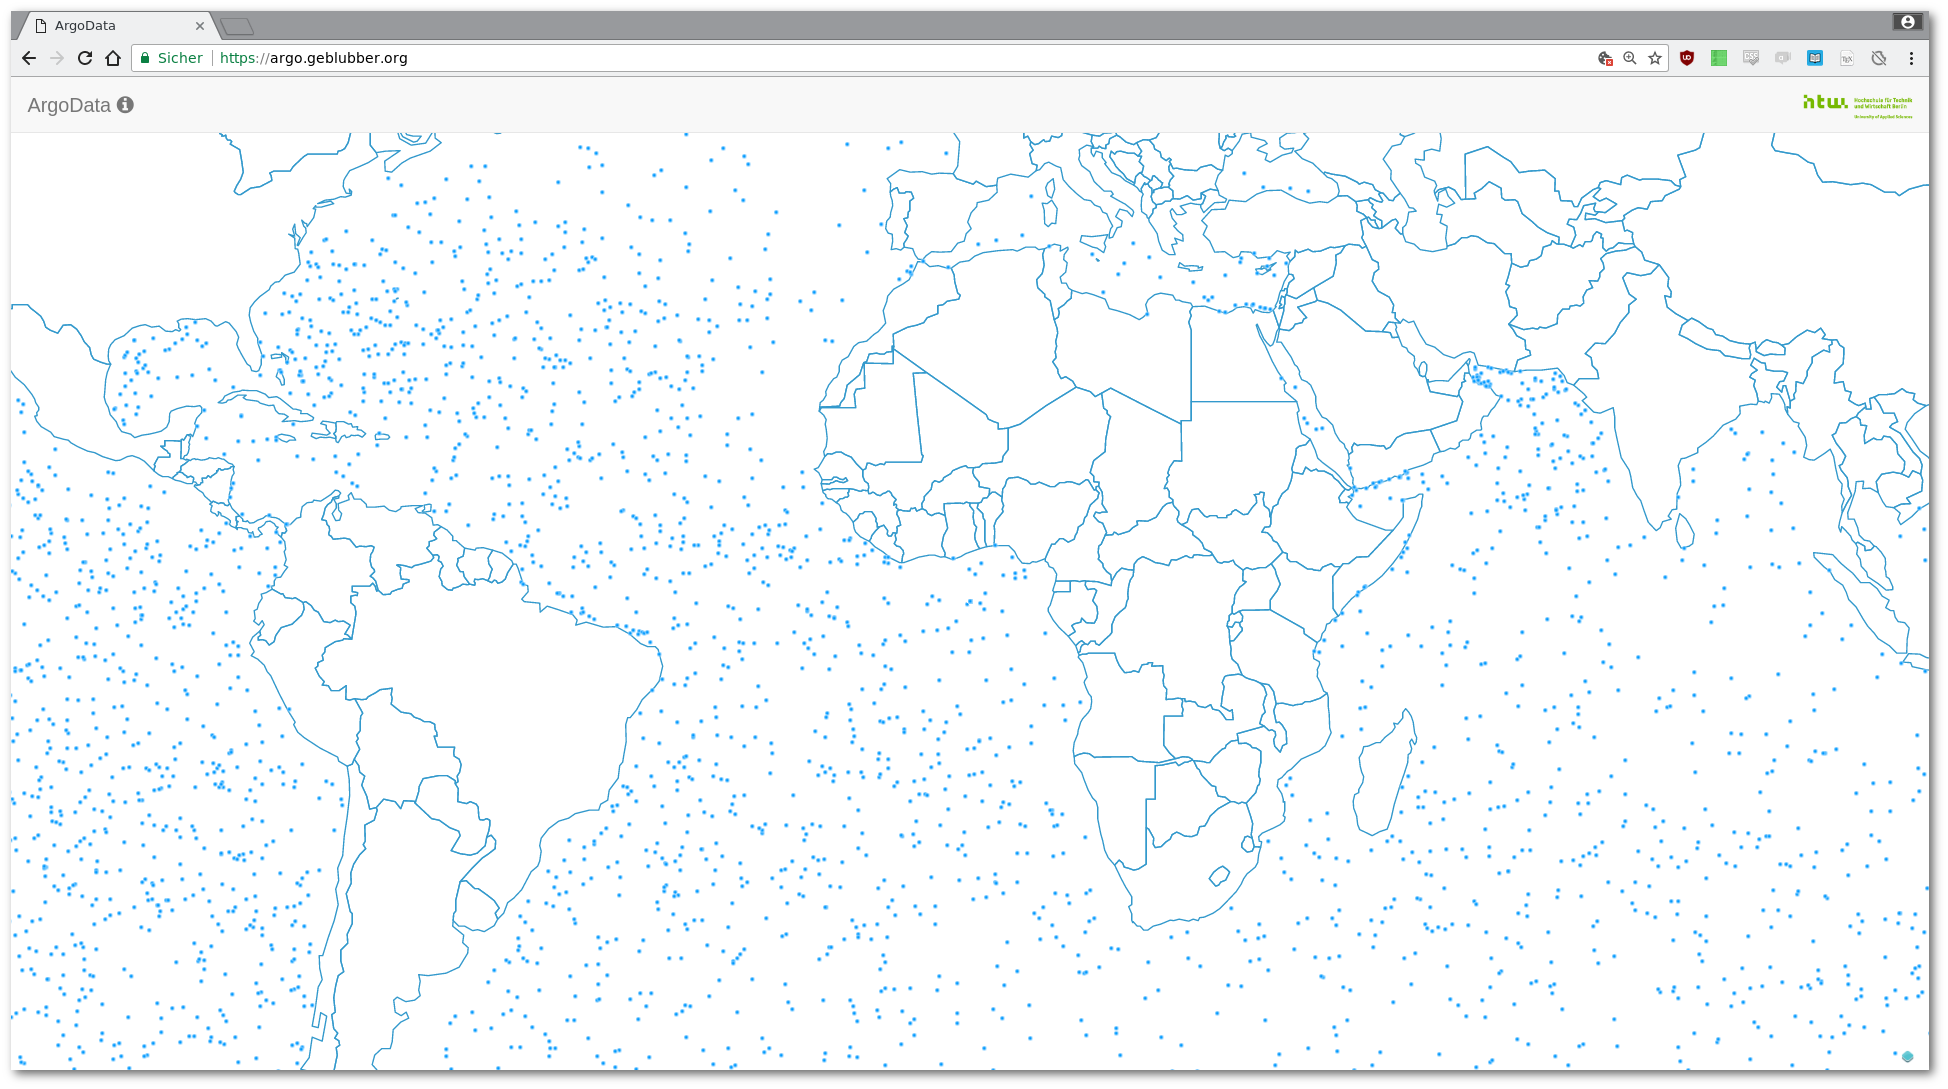
\includegraphics[width=0.39\textwidth]{pix/ftest/001.png}

 \caption{\textbf{Funktionstest I} Der Aufruf der Webapplikation}
 \label{fig:ftest001}
\end{wrapfigure}


Wie in Abbildung \ref{fig:ftest001} zu erkennen ist, werden die Grenzen der Ozeane und Kontinente über eine Weltkarte dargestellt, wenn die Webpräsenz der Applikation unter der für ArgoData registrierten Url aufgerufen wird. Die Karte ist über eine Vektorrepräsentation dargestellt, Landmarker wie Straßen und Städte sind darauf nicht zu erkennen. Die letzte Position der Messstationen ist über die jeweilige Position auf der Karte ersichtlich.
\newline\newline\newline


\begin{wrapfigure}[10]{l}{0.4\textwidth}
 \centering
 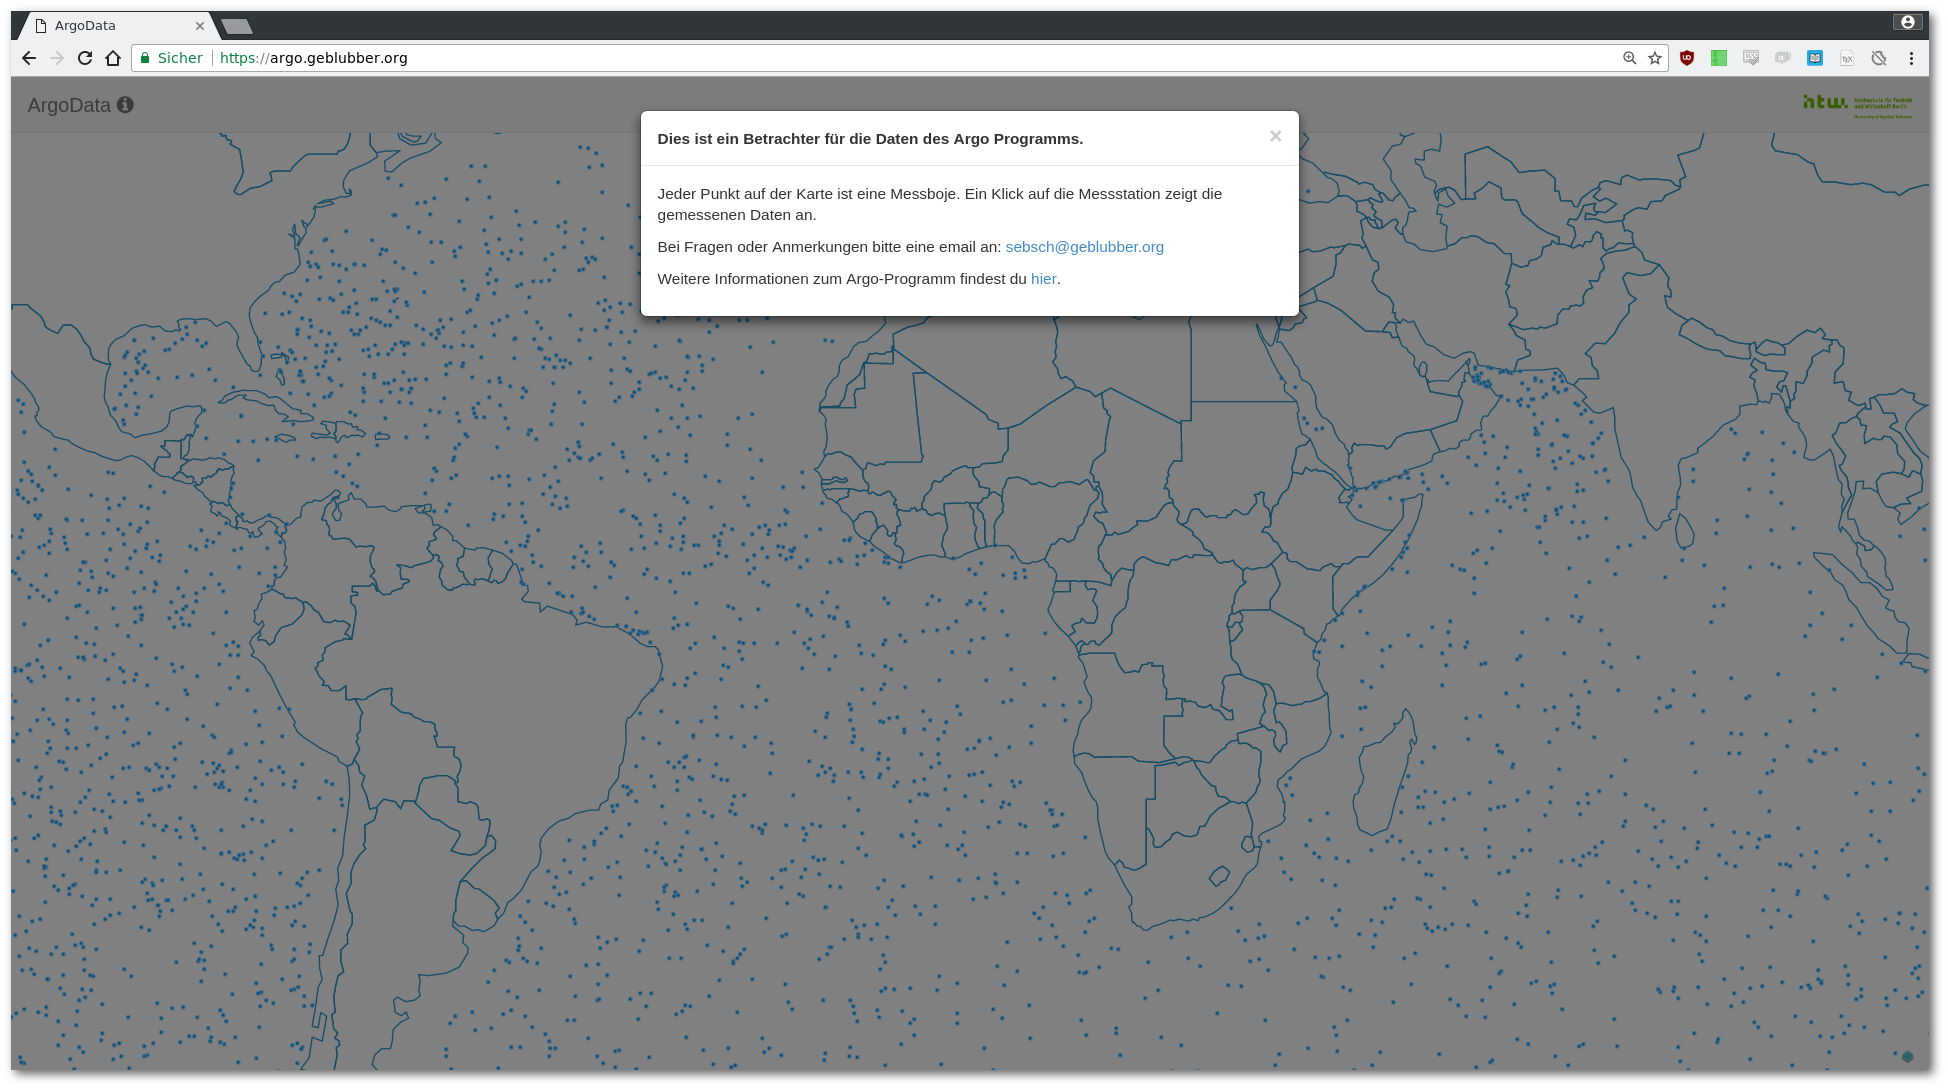
\includegraphics[width=0.39\textwidth]{pix/ftest/001b.png}
 \caption{\textbf{Funktionstest II} Die Anzeige der Hilfe}
 \label{fig:ftest001b}
\end{wrapfigure}

Durch Anklicken des Infobuttons erhält der Benutzer über ein Modal eine Kurzhilfe angezeigt. Diese erklärt die grundlegende Funktion der Webseite, stellt Kontaktdaten bereit und stellt über einen Web\-link eine Verbindung zum Argo-Programm her. In Abbildung \ref{fig:ftest001b} ist die Webseite mit aktiviertem Modal zu sehen.
\newline\newline\newline\newline \newpage


\begin{wrapfigure}[10]{l}{0.4\textwidth}
 \centering
 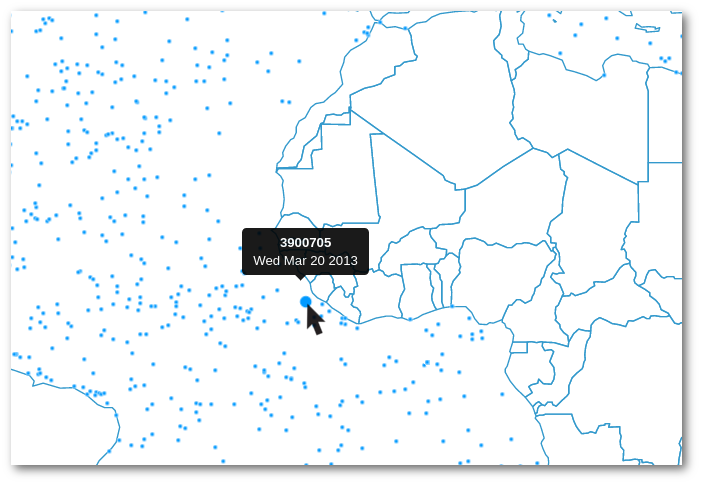
\includegraphics[width=0.39\textwidth]{pix/ftest/002.png}

 \caption{\textbf{Funktionstest III} Mousehover über Messstation}
 \label{fig:ftest002}
\end{wrapfigure}

Wird der Mauszeiger über die Repräsentation einer Messstation geführt, so erscheinen grundlegende Daten der Argo-Boje. Dies umfasst den eindeutigen Identifier sowie das Datum des letzten Messvorgangs. Zu erkennen in Abbildung \ref{fig:ftest002}.
\newline\newline\newline\newline\newline


\begin{wrapfigure}[10]{l}{0.4\textwidth}
 \centering
 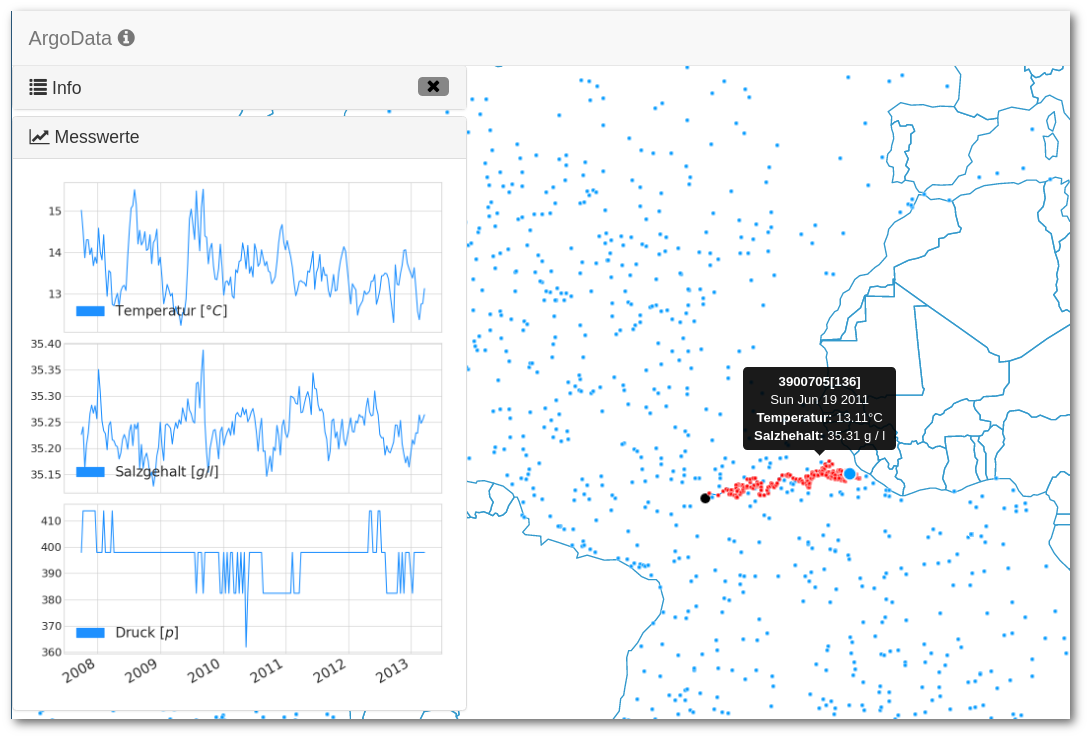
\includegraphics[width=0.39\textwidth]{pix/ftest/003.png}

 \caption{\textbf{Funktionstest IV} Werte werden angezeigt}
 \label{fig:ftest003}
\end{wrapfigure}

Durch einen Mausklick auf die Kartendarstellung der Argo-Boje werden weiterführende Daten angefordert. Wie in Abbildung \ref{fig:ftest003} zu sehen ist, werden  Messwerte  über Funktionsplots an der linken Seite der Webseite dargestellt. Dabei sind über die X-Achse der zeitliche Verlauf und über die Y-Achse der jeweilige Messwert kodiert. Die gemessenen Werte umfassen dabei Temperatur, Salzgehalt sowie Druck.  Der Ort der Messwerterhebung wird durch einen Punkt auf der Karte repräsentiert. Wird der Mauszeiger über diese Repräsentation geführt, werden neben dem Datum der Messung auch die gemessenen Werte dargestellt.

\newpage

\begin{wrapfigure}[10]{l}{0.4\textwidth}
 \centering
 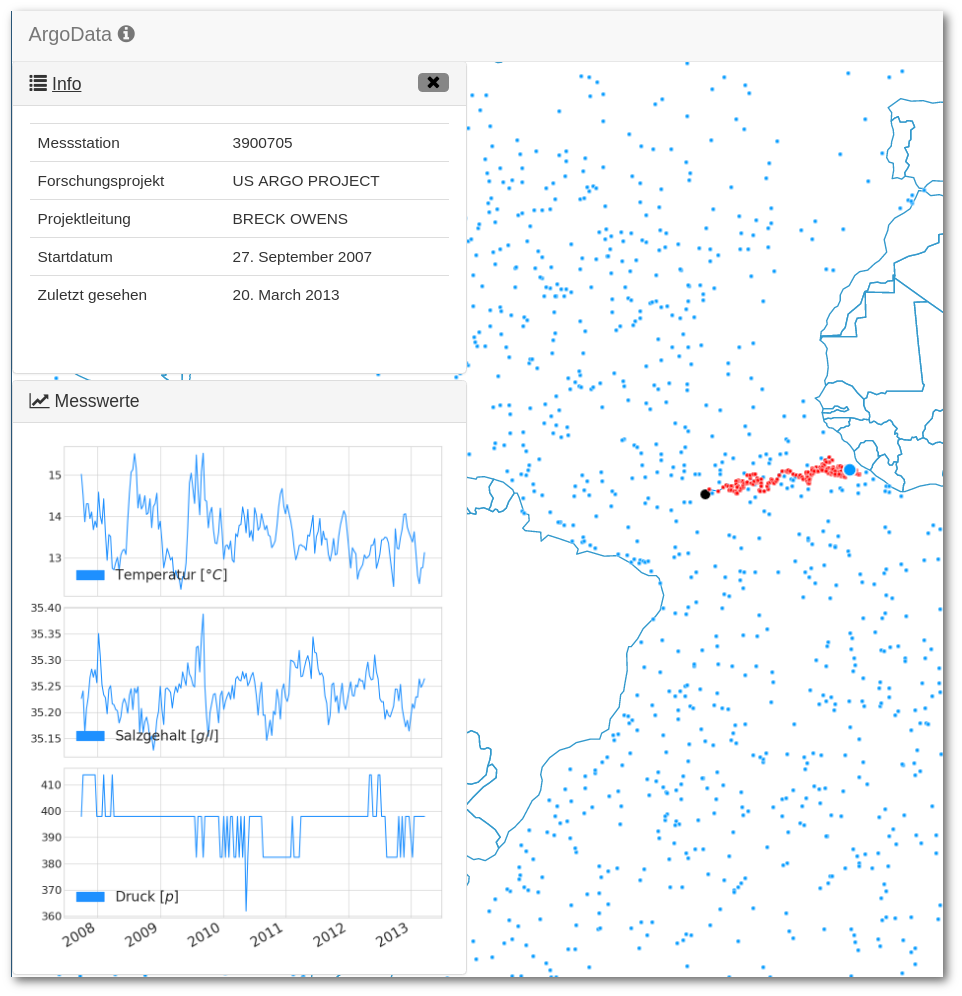
\includegraphics[width=0.35\textwidth]{pix/ftest/003b.png}

 \caption{\textbf{Funktionstest V} Metainformationen werden angezeigt}
 \label{fig:ftest003b}
\end{wrapfigure}

Wird der Reiter "`Info"' angeklickt, so werden weitere Informationen zur Messstation sichtbar. Wie in Abbildung \ref{fig:ftest003b} zu sehen ist,  Umfassen diese den Identifier der Messstation, das verantwortliche Forschungsprojekt, den Besitzer der Boje sowie das Startdatum und das Datum der letzten Messung.
\newline\newline\newline\newline
\newline\newline\newline


\begin{wrapfigure}[10]{l}{0.4\textwidth}
 \centering
 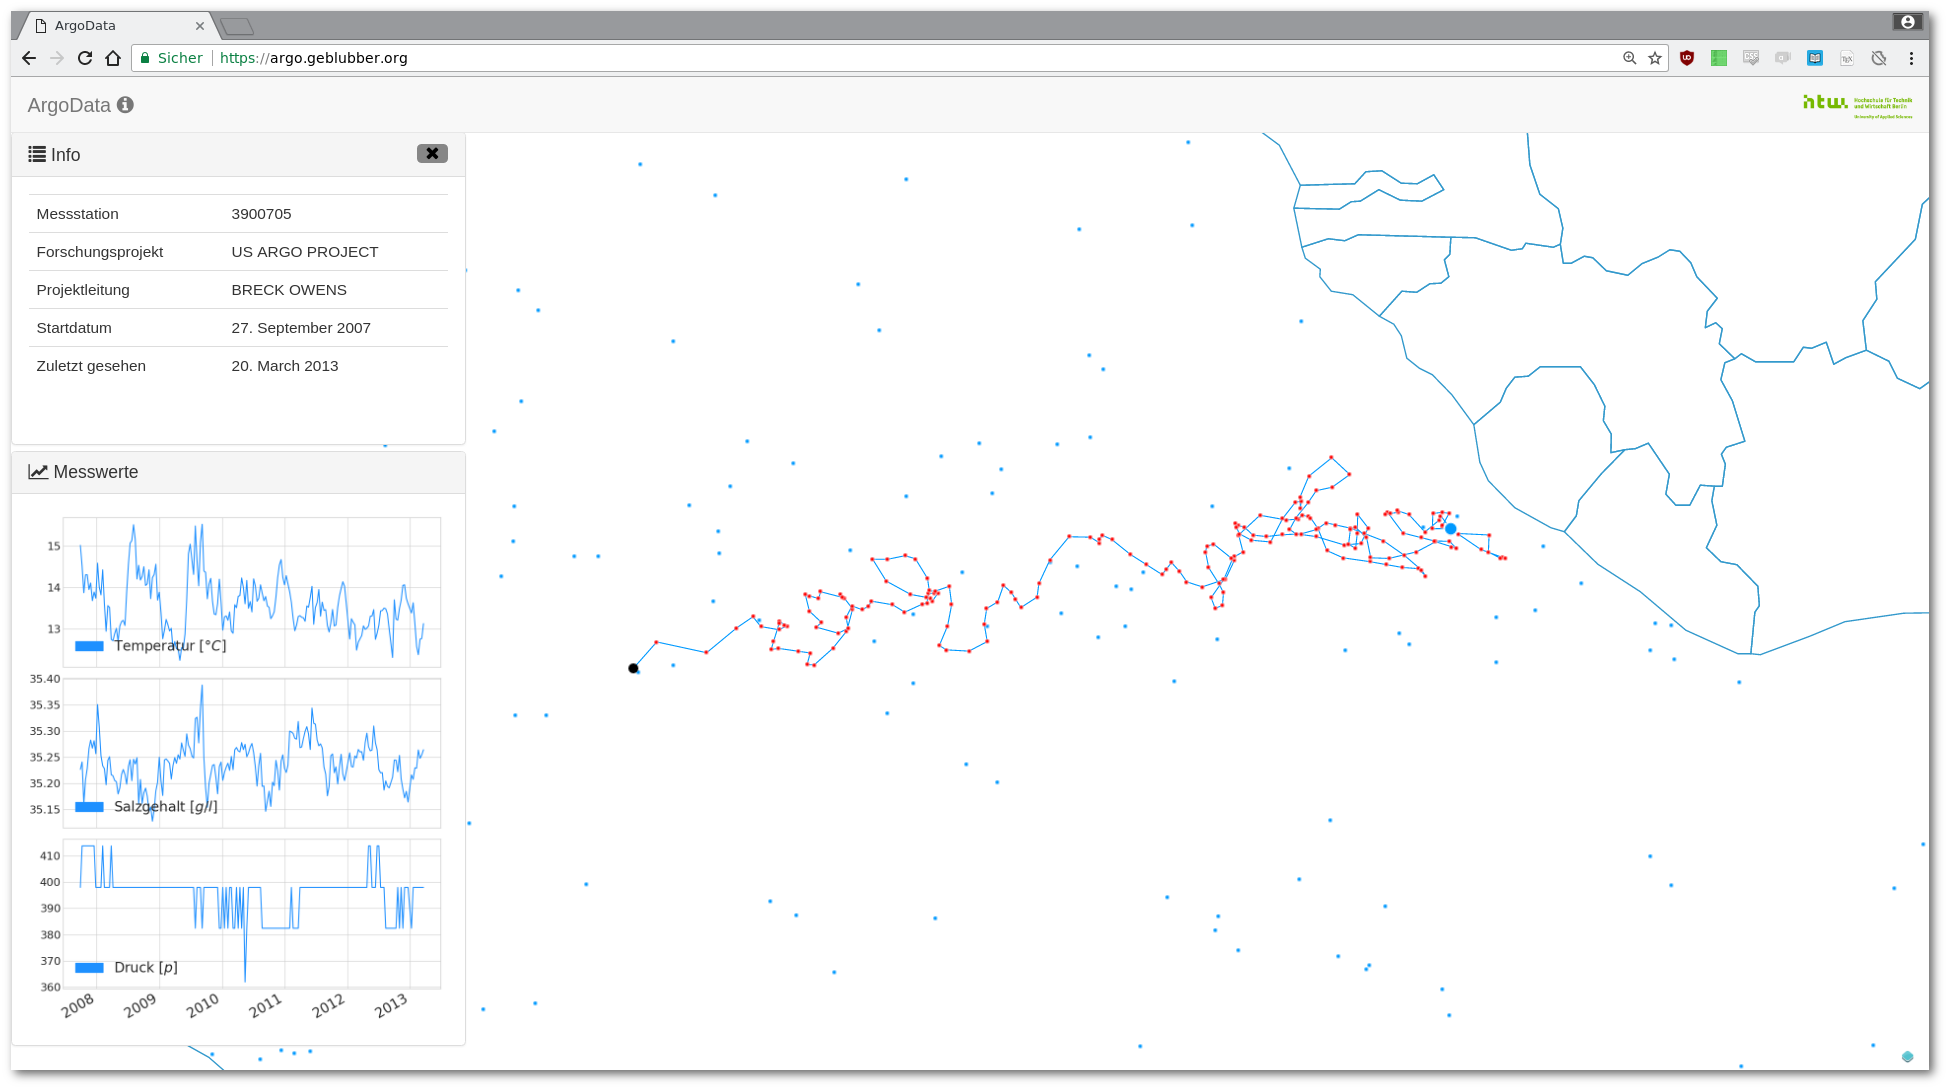
\includegraphics[width=0.35\textwidth]{pix/ftest/004.png}

 \caption{\textbf{Funktionstest VI} Der Pfad der Messstatioon kann zurückverfolgt werden}
 \label{fig:ftest004}
\end{wrapfigure}

Wie in Abbildung \ref{fig:ftest004} zu erkennen ist, wird der zwischen zwei Messpunkten der zurückgelegte Weg über eine Linie dargestellt. Somit kann der Weg, den eine Messstation zurückgelegt hat um die Daten zu erheben, klar nachvollzogen werden.
\newline\newline\newline\newline
\newline\newline\newline


\begin{wrapfigure}[10]{l}{0.4\textwidth}
 \centering
 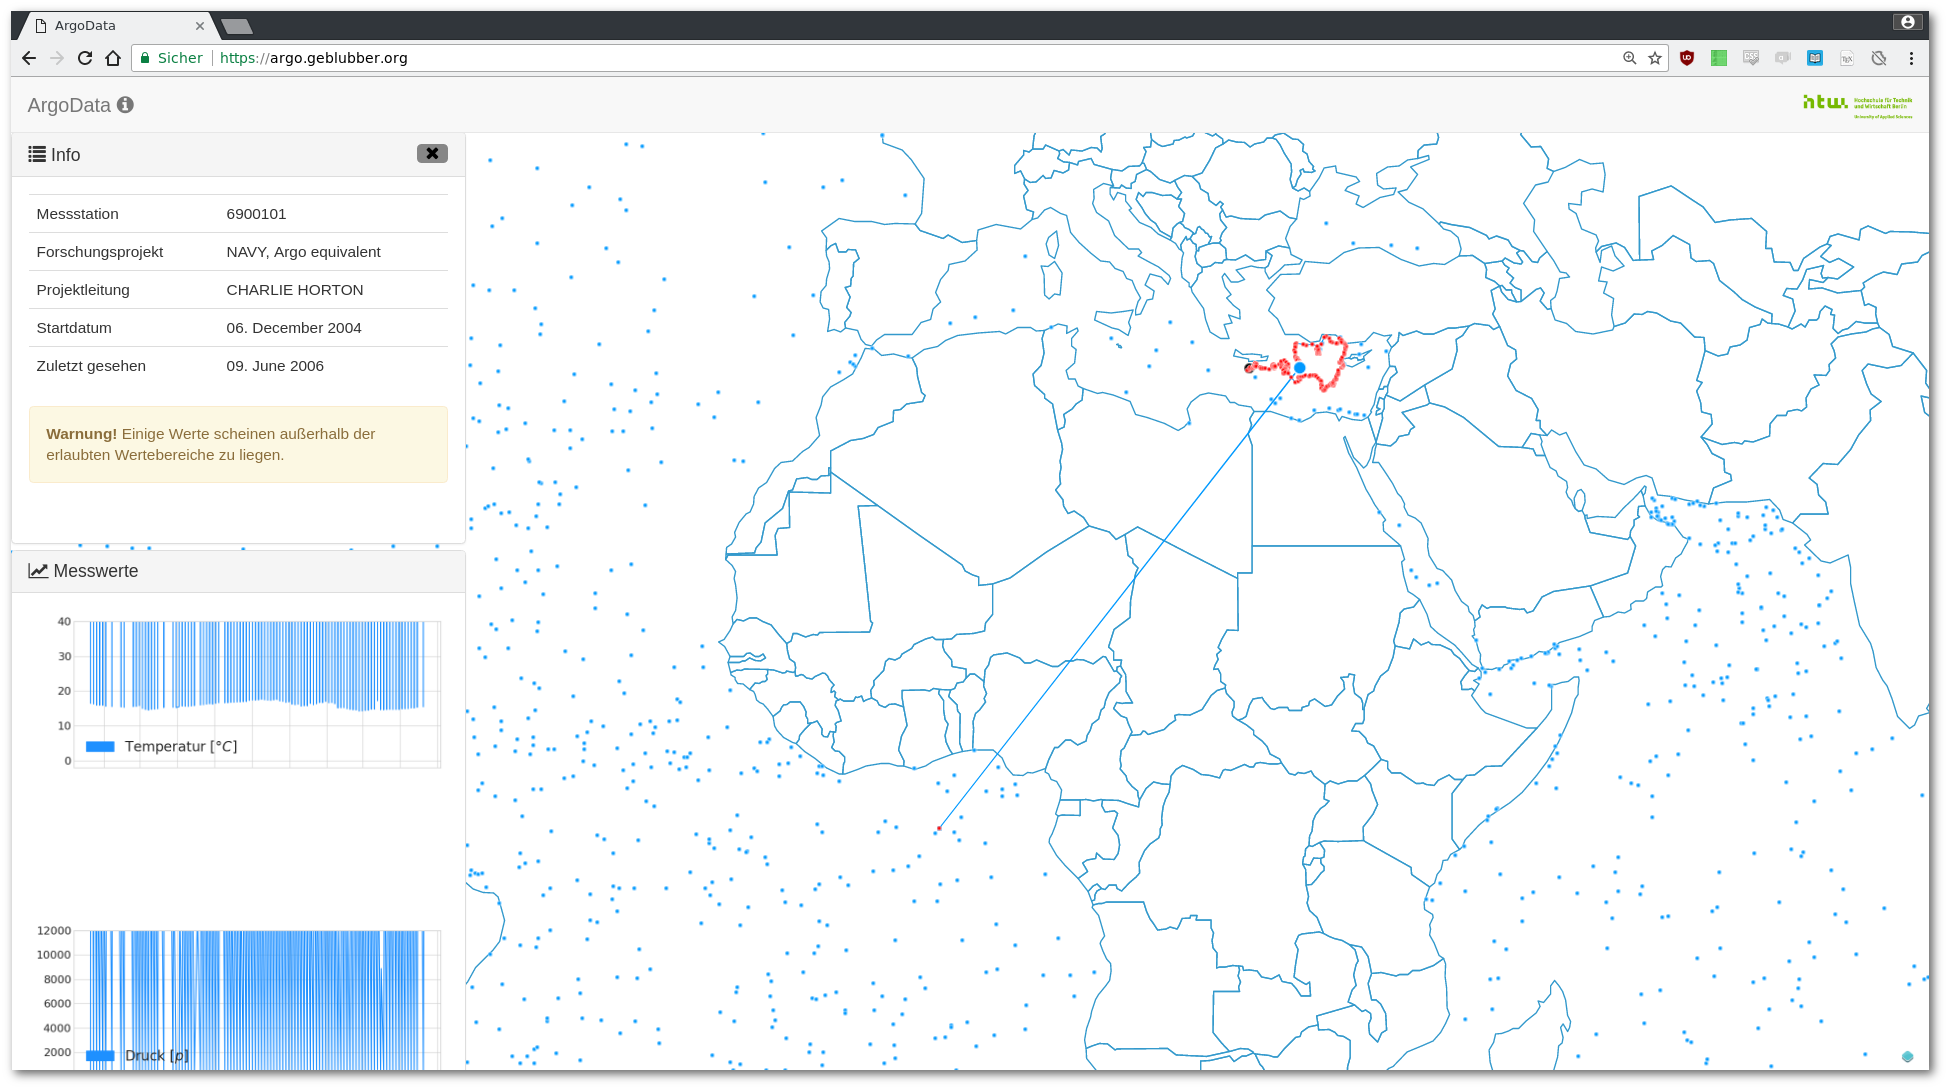
\includegraphics[width=0.35\textwidth]{pix/ftest/00fail.png}

 \caption{\textbf{Funktionstest VI} Fehlerhafte Daten werden markiert}
 \label{fig:ftest00fail}
\end{wrapfigure}

In Abbildung \ref{fig:ftest00fail} ist ersichtlich, dass fehlerhafte Daten durch eine Warnung hervorgehoben werden. Diese informiert die Benutzenden, dass die Daten, die gerade angezeigt werden, zum Teil die Wertebereiche überschritten haben. Die Achsen der Funktionsplots werden auf die Wertebereiche beschränkt und Plots von mit \texttt{nan} kodierten Messwerten nicht dargestellt.
\newline
\newline



\subsubsection{Aggregation der Daten}

In Listing \ref{lst:renewdatash} ist der Prozess der Datenerneuerung zu sehen. Dieser Umfasst die in Kapitel \ref{sec:funkAnforderungenAdmin} festgelegten Anforderungen. Der Ablauf ist im Folgenden beschrieben.

\begin{python}[%
        label={lst:renewdatash},%
        caption={Erneuerung des Datensatzes}]
 -> # bash /root/argo_proto/renew_data.sh
(!) Starting renew process at Tue Mar  6 12:41:24 CET 2018.
 >> Downloading new data...
        done.
Datafolder: /root/aoml/
||||||||||||||||||||||||||||||||||| 6711/6711 [2:02:33<00:00,  1.10s/it]
 >> Dumping tmpdb to /tmp/argo_db.sql ...
        done. [164601410 Mar  6 14:44 /tmp/argo_db.sql]
 >> Renew production database ...
        done.
 >> Renew Argos cache...
        done.

Process finished.
This took  7381 seconds.
We had a downtime of 11 seconds.
So long and thanks for all the fish. Bye.
\end{python}

\begin{description}
 \item [Daten herunterladen]
    Die Daten des Argo-Programms werden heruntergeladen. Es handelt sich um die Livedaten nach der Qualitätskontrolle aus der Quelle \texttt{aoml}. Für das herunterladen wird rsync verwendet. In der Quelle nicht mehr vorhandene Daten werden gelöscht.


 \item [Daten aggregieren]
    Der Aggregationsteil der hier entwickelten Software wird verwendet, die soeben erneuerten Daten in die Datenbank zu überführen. Um Ausfallzeiten der Webapplikation möglichst gering zu halten, werden die Daten zunächst in eine temporäre Datenbank geschrieben. Über einen Ladebalken wird der derzeitige Stand dieses Prozesses sichtbar. Es ist außerdem ersichtlich, dass die Daten von 6711 Messstationen in 2 Stunden, 2 Minuten und 30 Sekunden in die Datenbank überführt wurden.

 \item [Erstellen eines Datenbankdumps]
    Um die Daten in die Produktionsdatenbank zu überführen, werden die Tabellen der temporären Datenbank gedumpt. Es ist ersichtlich, dass der Dump eine Größe von  ca. 20 Megabyte umfasst.

 \item [Einspielen des Datenbankdumps]
    Über die Funktionalitäten des Postgresql-Clients \texttt{psql} werden die Daten in die Produktionsdatenbank überführt. Dieser Prozess erfordert eine Ausfallzeit der Webapplikation von 11 Sekunden.

 \item [Erneuern des Caches zur Anzeige der Argo-Floats]
    Um die Daten in der Anzeige zu erneuern, wird der Cache neu geschrieben. Für diesen Zweck wird ein GET-Request an die hierfür festgelegte URL gesendet. Die Webapplikation erneuert daraufhin den Cache. Damit stehen der Webapplikation die erneuerten  Daten zur Verfügung.
\end{description}



\newpage
\subsection{Usability-Umfrage}

\subsubsection{Testaufbau}

Um die Usability der Webapplikation zu testen, wurde eine Umfrage durchgeführt. Als Grundlage diente der System Usability Scale (SUS).
Für diese Umfrage waren insgesamt 10 Fragen innerhalb einer Scala von 0 (gar nicht) bis 5 (sehr)  zu bewerten. (vgl. \cite{Quantita52:online})

An der Umfrage nahmen insgesamt 12 Personen teil. Diese setzen sich aus Bekannten- und Kollegenkreis zusammen. Die Daten wurden anonym erhoben, ein Rückschluss auf die Personen ist damit nicht mehr möglich.

In Abbildung \ref{fig:surveyAuswertung}
ist eine grafische Zusammenfassung der Ergebnisse zu sehen. In dieser findet sich zu jeder Frage ein Balkendiagram der akkumulierten Häufigkeit, kombiniert mit einem Box-Whisker-Plot. Dieser setzt sich aus folgenden Elementen zusammen:

\begin{description}
 \item [Box]
    Dies markiert den Bereich in welchem sich 50\% der Daten finden. Der Median wird durch eine vertikale Linie gezeigt. Die hier vorliegende Darstellung ist um den Mittelwert (mean) erweitert. Die schmale Linie stellt das arithmetische Mittel und die fett gedruckte den Median dar.
 \item [Whisker (Antennen)]
    Dieser Bereich stellt die äußeren Quantile dar. In der Grundeinstellung 1.5 wird die von John W. Turkey verwendete Einstellung von maximal dem 1.5-fachen des Interquartilabstandes für den Whiskerbereich verwendet.
\end{description}


\subsubsection{Testauswertung}

Im Folgenden findet sich eine detaillierte Auswertung der hier erhobenen Daten:


\paragraph{\texttt{Statement 1:} "`Ich kann mir gut vorstellen, ArgoData regelmäßig zu nutzen."'}
    Diese Frage zielt auf die Wiederbesuchsbereitschaft ab. 
    
    Die Antworten weisen eine breite Streuung auf. 
    In insgesamt 4 von 5 Antwortmöglichkeiten wurden Antworten gegeben. 
    4 von 12 Personen bewertenden das Statement mit einem Wert von 4.
    Der Median liegt bei 3, der Durchschnitt zwischen 2.5 und 3. Die Box umfasst die Antworten 2 bis 4. Der Whisker schließt Antwort 1 mit ein.

 \paragraph{\texttt{Statement 2:} "`Ich empfinde ArgoData als unnötig komplex."'}
    In dieser Frage, bildet sich die Reduktion der Komplexität ab. Dire Antworten finden sich hier im bereich 1 bis 3. Das Maximum liegt mit einem Wert von 7 in der Antwort 1. Der Median liegt bei 1, das arithmetische Mittel bei knapp über 1.5. Die Box umfasst die Antworten 1 bis 2. Der Whisker schließt Antwort 3 mit ein.

  \paragraph{\texttt{Statement 3:} "`Ich empfinde ArgoData als einfach zu nutzen."'}
    Durch diese Frage wird die Einfachheit der Darstellung und die Reduktion der Benutzungskomplexität abgebildet. Die Antworten finden sich hier im Bereich 3 bis 5. Das Maximum liegt mit 6 Antworten klar bei Antwort 5. Die Box umfasst Antworten 4 und 5. Der Whisker schließt Antwort 3 mit ein.

\paragraph{\texttt{Statement 4:} "`Ich denke, dass ich Hilfestellung bei der Benutzung brauchen würde um ArgoData zu benutzen."'}
    Diese Frage ermittelt ob genügend Hilfestellung zur Verfügung gestellt wurde.  Die Antworten finden sich im Bereich 1 bis 4. Das Maximum von 4 findet sich in den Antworten 1 und 3.  Der Median liegt bei 2.5, das arithmetische Mittel liegt zwischen 2.5 und 2. Die Box umfasst Antworten 1 bis 3, der Whisker schließt Antwort 4 mit ein.

\paragraph{\texttt{Statement 5:} "`Ich finde, dass die Funktionen (Karte, Steuerung, Anzeige von Daten) gut integriert sind."'}
    Diese Frage ermittelt die Integration der Steuerungselemente. Hier finden sich die Antworten zwischen 3 und 5. Das Maximum liegt mit einem Wert von 6 bei Antwort 4. Der Median liegt bei 4, das arithmetische Mittel zwischen 4 und 4.5. Die Box umfasst  die Antworten 4 und 5. Der Whisker schließt Antwort 3 mit ein.

\paragraph{\texttt{Statement 6:} "`Ich finde, dass es in ArgoData zu viele Inkonsistenzen gibt."'}
    Diese Frage zielt auf die Integration der Komponenten als Gesamtkonzept ab. Die Antworten finden sich von 1 bis 3. Das Maximum liegt mit 5 bei Antwort 2. Der Median liegt bei 2, das arithmetische Mittel liegt leicht darüber. Die Box umfasst Antworten 2 und 3. Der Whisker schließt Antwort 1 mit ein.

\paragraph{\texttt{Statement 7:} "`Ich kann mir vorstellen, dass die meisten Leute ArgoData schnell zu beherrschen lernen."'}
    Diese Frage versucht über eine extrene Perspektive die Lernkurve bei der Benutzung abzufragen. Die Antworten finden sich im Bereich 3 bis 5. Das Maximum liegt mit 6 bei Antwort 5. Der Median liegt bei 4.5, das arithmetische Mittel liegt knapp darunter. Die Box umfasst die Antworten 4 und 5. Der Whisker schließt Antwort 3 mit ein.

\paragraph{\texttt{Statement 8:} "`Ich empfinde die Bedienung als sehr umständlich."'}
    Diese Frage versucht das Erleben des Bedienungskonzeptes zu erfragen. Die Antworten finden sich im Bereich 1 bis 3. Das Maximum liegt mit 7 bei Antwort 2. Der Median liegt bei 2, das arithmetische Mittel im Bereich zwischen 1.5 und 2. Die Box umfasst die Antworten 1 und 2. Der Whisker schließt Antwort 3 mit ein.

\paragraph{\texttt{Statement 9:} "`Ich musste eine Menge Dinge lernen, bevor ich mit ArgoData arbeiten konnte."'}
    Diese Frage ermittelt die Lernkurve die zur Benutzung notwendig ist. Hier finden sich die Antworten im Bereich von 1 bis 4. Das Maximum liegt mit 9 von 12 Antworten bei 1. Der Median liegt bei Antwort 1, das arithmetische Mittel bei ca. 1.5. Die Box umfasst Antwort 1, der Whisker schließt keine weiteren Antworten mit ein, diese sind damit als Ausreißer zu betrachten.

\subsubsection{Interpretation der Ergebnisse}
Die Antworten sind durchwegs als positiv zu betrachten. Die Fragen zur Komplexität lassen erkennen, dass es gelungen ist, die wissenschaftlichen Daten ohne Vorkenntnisse verstehbar darzustellen. Die Bedienungsmuster wurden angenommen und als konsistent und wenig umständlich beschrieben. Die Frage zur Wiederbesuchsbereitschaft weist eine starke Streuung auf. Da es sich um eine Seite mit einem Bildungsangebot handelt, ist dies erklärbar.
Ein klarer Verbesserungswunsch lässt sich aus der Frage zu den angebotenen Hilfestellungen ableiten. Hier gilt es  zu überlegen, ob und in welcher Form den benutzenden Personen zur Hand gegangen werden kann.



\begin{figure}
 \centering
 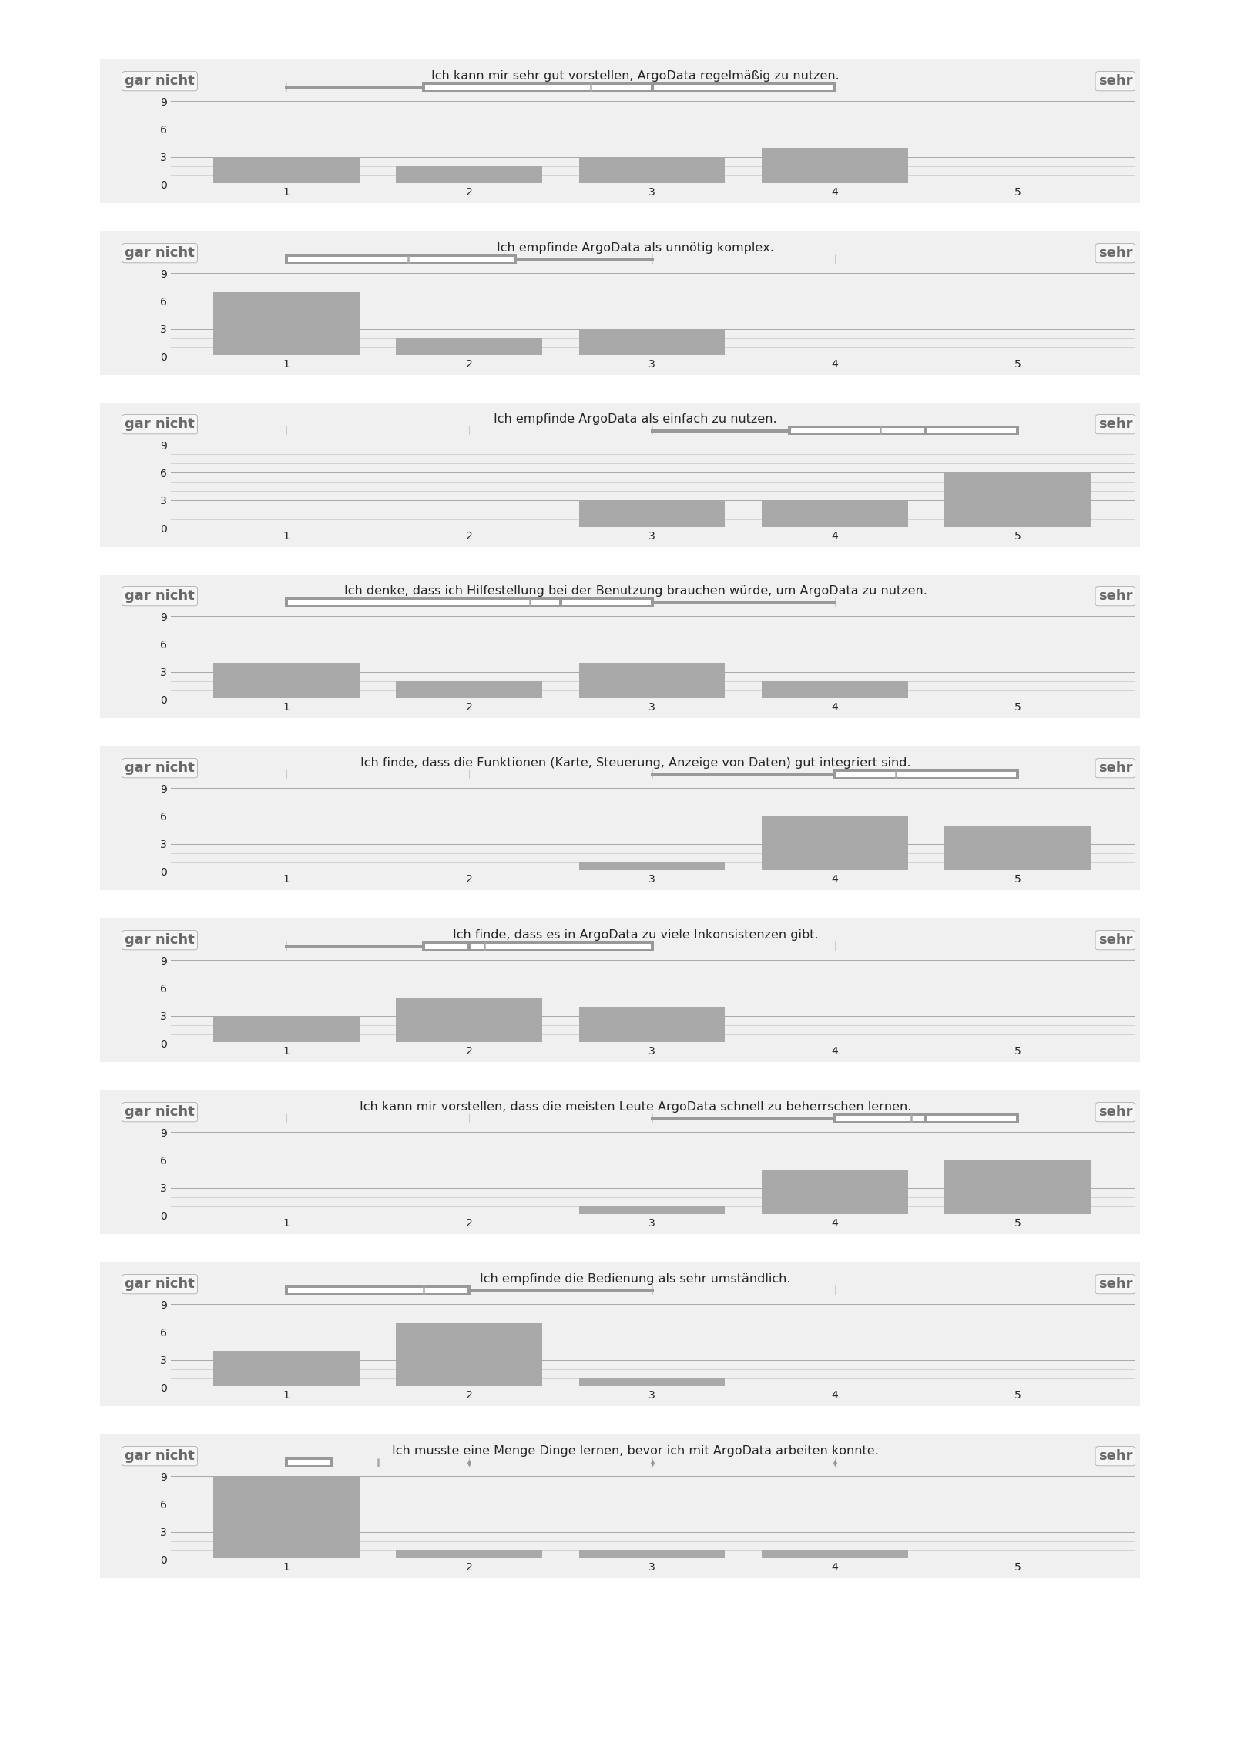
\includegraphics[width=\textwidth,height=0.98\textheight,clip=true,trim=2cm 3cm 1.6cm 1cm]{pix/surveyAuswertung.pdf}

 \label{fig:surveyAuswertung}
 \caption{Ergebnis der Umfrage zur Usability}
\end{figure}
